\section{Parallelization performance}
\label{sec:dsmc_parallelization_performance}
No matter how many processors we distribute the work load to, the total computation time needed to perform a simulation is obviously not reduced. There are still as many collisions as before as the physical problem is identical. The idea is to do many calculations at the same time so that the \textit{real} time we actually wait is reduced. Parallelizing comes with a cost, as we need more logic to allow the processors communicate with each other (exchanging particles and waiting for each other to finish each time step). As the number of processors increases, the total computation time \textit{per processor} is reduced, but the time spent on communication often increases. We will measure what's called \textit{parallel scalability} which indicates how efficient a program is when the number of processors is increased. There are two different kinds of scalability - weak and strong scaling
\begin{itemize}
	\item strong scaling is how the computation time changes with an increased number of processors on a fixed system size, whereas the
	\item weak scaling is how the computation time changes with an increased number of processors on a fixed system size \textit{per processor}.
\end{itemize}
\subsection{Strong scaling}
To see how the program efficiency scales with a fixed system size while increasing the number of processors is important if we want to study a specific system (a given system size and geometry, e.g. scanned from real data), but we would like to reduce the simulation run time. With a fixed system size, the total number of particles per CPU is reduced while increasing the total number of processors. We define the \textit{strong scaling efficiency} $\eta_s$ as
\begin{align}
	\eta_s = \frac{t_1}{Nt_N},
\end{align}
where $t_1$ is the total run time using one processor and $t_N$ is the total run time using $N$ processors. We see that $\eta_s\in (0,1)$ since $Nt_N$ is the ideal scaling without any communication overhead. In this benchmark, we have run the simulation in an empty geometry - there are no surfaces to collide with. The physical system is a cube with side length $L=$\unit{1.0}{\micro\meter} with a density $\rho_n=\unit{1.0\e{27}}{\meter^{-3}}$ which gives a total of one billion atoms. We choose that one DSMC particle represents 50 atoms, yielding a total of 20 million particles in the whole system. The benchmark was performed for 10000 timesteps ($\Delta t = 0.005$) with $2^N$ processors from 1 CPU to 512 CPUs yielding a good estimate of how efficient the program scales for a relatively large number of processors. In table \ref{tab:dsmc_strong_scaling} we have the scaling results with additional information like the number of intermolecular collisions per processor. This indicates the amount of computation each processor has to perform. The strong scaling efficiency is plotted together with the weak scaling against the number of processors in figure \ref{fig:dsmc_scaling}. We see that the program scales great with only 30\% overhead for 512 processors. The weird behavior we see at 128 processors, where the efficiency \textit{increases} to 0.9, is probably due to random \"luck\" on the supercomputer where all nodes are physically close to each other. In order to get better statistics, this benchmark should be run several times.
\begin{table}[h]
\begin{center}
    \begin{tabular}{|l|l|l|l|l|l}
    \hline
    $N_\text{CPU}$ & $N_\text{particles}/N_\text{CPU}$ & $N_\text{collisions}/N_\text{CPU}$ & $t_n$ [s] & $\eta_s$ \\ \hline
    1 & 2.0\e{7} & 1.16\e{11} & \unit{90802}{\second} & 1.0\\
    \hline
    8 & 2.5\e{6} & 1.45\e{10} &  \unit{15372}{\second} & 0.74\\
    \hline
    16 & 1.25\e{6} & 7.25\e{9} &  \unit{6752}{\second} & 0.84\\
    \hline
    32 & 6.3\e{5} & 3.62\e{9} &  \unit{3805}{\second} & 0.75\\
    \hline
    64 & 3.1\e{5} & 1.81\e{9} &  \unit{1706}{\second} & 0.83\\
    \hline
    128 & 1.6\e{5} & 9.06\e{8} &  \unit{785}{\second} & 0.90\\
    \hline
    256 & 7.8\e{4} & 4.53\e{8} &  \unit{415}{\second} & 0.85\\
    \hline
    512 & 3.9\e{4} & 2.27\e{8} &  \unit{250}{\second} & 0.71\\
    \hline
    \end{tabular}
    \caption{Benchmark results showing the strong scaling efficiency $\eta_s$ for the DSMC program. We see that the program scales great with only 30\% overhead for 512 processors. The weird behavior we see at 128 processors, where the efficiency \textit{increases} to 0.9, is probably due to random \"luck\" on the supercomputer where all nodes are physically close to each other. In order to get better statistics, this benchmark should be run several times.}
    \label{tab:dsmc_strong_scaling}
    \end{center}
\end{table}

\subsection{Weak scaling}
Another important scaling problem appears when we want to maximize the simulated system size. If we keep a constant system size \textit{per CPU}, and increase the number of processors, the limitation of how big we efficiently can create the system is controlled by the weak scaling. We then introduce the \textit{weak scaling efficiency} $\eta_w$ defined as
\begin{align}
	\eta_w = \frac{t_1}{t_N},
\end{align}
where again $t_1$ is the total run time using one processor and $t_N$ is the run time using $N$ processors. If the algorithm scales perfectly, the total run time would remain constant while increasing the number of processors (each CPU is ideally independent), but we expect some overhead. This implies that the range for $\eta_w$ also is between zero and one. We have run the same geometry as for the strong scaling, but each processor controls a volume of \unit{1}{\micro\meter^3} so that the largest system is \unit{512}{\micro\meter^3}. Keeping the same density, but using 500 atoms per particle, gives a total of 2 million particles per processor. In table \ref{tab:dsmc_weak_scaling} and figure \ref{fig:dsmc_scaling}, we see the results for the weak scaling efficiency simulation. The weak scaling also shows promising results with a reasonable low overhead.
\begin{table}[h]
\begin{center}
    \begin{tabular}{|l|l|l|l|l|l}
    \hline
    $N_\text{CPU}$ & $N_\text{particles}$ & $N_\text{collisions}$ & $t_N$ & $\eta_w$ \\ 
    \hline
    1 & 2.00\e{6} & 5.83\e{9} & \unit{3450}{\second} & 1.0\\
    \hline
    2 & 4.00\e{6} & 1.16\e{10} & \unit{3640}{\second} & 0.95\\
    \hline
    4 & 8.00\e{6} & 2.33\e{10} & \unit{5190}{\second} & 0.67\\
    \hline
    8 & 1.60\e{7} & 4.66\e{10} & \unit{4700}{\second} & 0.73\\
    \hline
    16 & 3.20\e{7} & 9.31\e{10} & \unit{6620}{\second} & 0.52\\
    \hline
    32 & 6.40\e{7} & 1.86\e{11} & \unit{5470}{\second} & 0.63\\
    \hline
    64 & 1.28\e{8} & 3.73\e{11} & \unit{5360}{\second} & 0.64\\
    \hline
    128 & 2.56\e{8} & 7.45\e{11} & \unit{5760}{\second} & 0.60\\
    \hline
    256 & 5.12\e{8} & 1.49\e{12} & \unit{5430}{\second} & 0.64\\
    \hline
    512 & 1.02\e{9} & 2.98\e{12} & \unit{5450}{\second} & 0.63\\
    \hline
    \end{tabular}
    \caption{Benchmark results showing the weak scaling efficiency $\eta_w$ for the DSMC program.}
    \label{tab:dsmc_weak_scaling}
    \end{center}
\end{table}

\begin{figure}[h]
\begin{center}
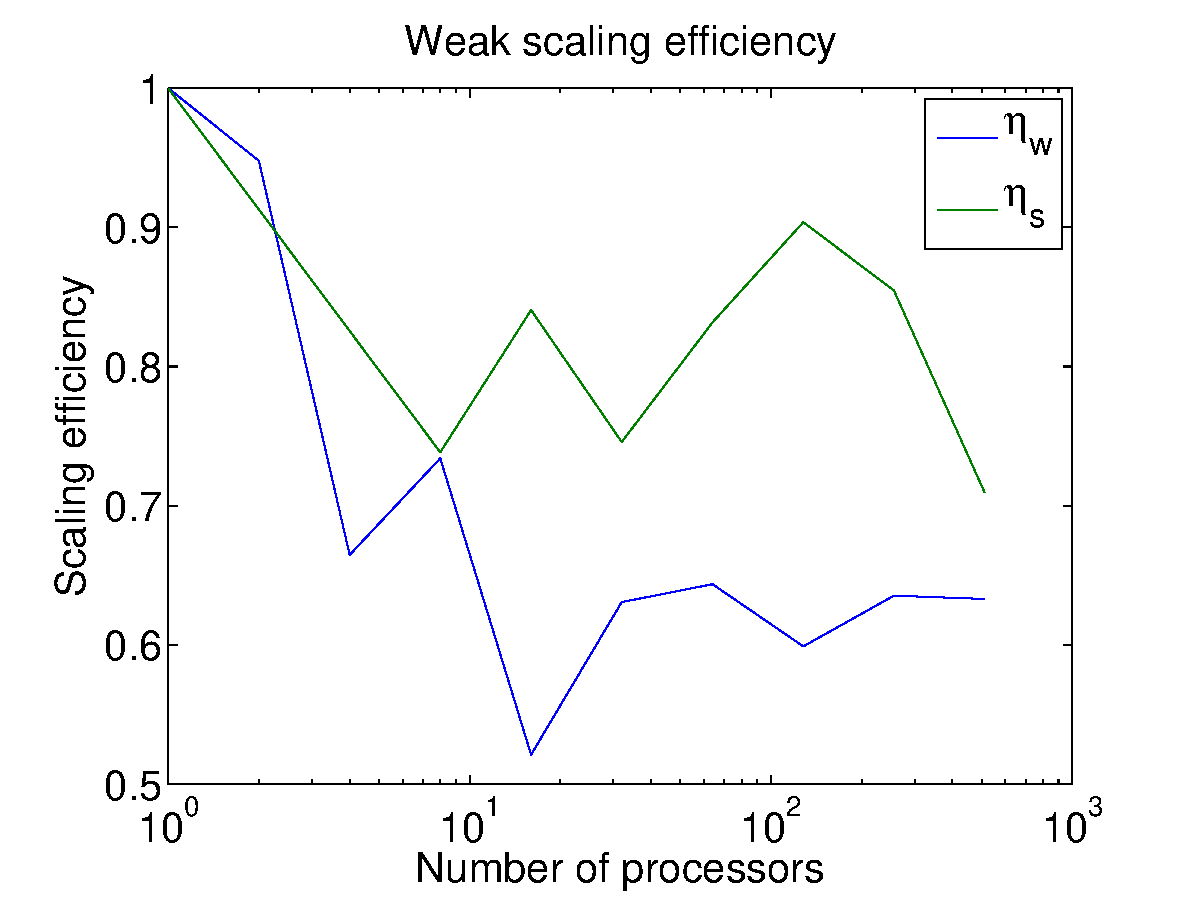
\includegraphics[width=\textwidth, trim=0cm 0cm 0cm 0cm, clip]{DSMC/figures/scaling.eps}
\end{center}
\caption{The weak and strong scaling efficiency, $\eta_w$ and $\eta_s$, as a function of the number of processors $N_\text{CPU}$. We see that at 512 processors, both efficiencies are reduced to 60-70\% because of the MPI communication overhead. Despite the bad statistics, it seems like the efficiency has more or less converged to a satisfactory level.}
\label{fig:dsmc_scaling}
\end{figure}

\section{Results for simple geometries}
\label{sec:results_for_simple_geometries}
In this section, we study flow in a simple geometry where the permeability is known from theory. The expression for the permeability is only valid for small Knudsen numbers (which we called the absolute permeability; the permeability for fluids in the continuum limit), so it is a perfect test case for the Knudsen correction factor $f_c$ in equation \eqref{eq:knudsen_correction}. 
\subsection{Flow in a cylinder, varying Knudsen number}
We have induced flow in a cylinder with radius \unit{0.45}{\micro\meter} with an applied acceleration corresponding to a pressure difference $\Delta P = 0.1P_0$, where $P_0$ is the ideal gas pressure at \unit{300}{\kelvin}. While varying the density, we adjusted $N_\text{eff}$ so that the total number of simulated particles was approximately one million. We expect an apparent permeability satisfying the Knudsen correction
\begin{align}
	k_a = k_\infty f_c = k_\infty[1 + \alpha(\text{Kn})\text{Kn}]\left[1 + {4\text{Kn}\over 1 + \text{Kn}}\right].
\end{align}
The analytical absolute permeability for a cylinder with radius $r$ is given by\cite{karniadakis2005microflows}
\begin{align}
	\label{eq:permeability_cylinder}
	k_\infty = {r^2\over 8},
\end{align}
which gives the following prediction for the apparent permeability
\begin{align}
	k_a = [1 + \alpha(\text{Kn})\text{Kn}]\left[1 + {4\text{Kn}\over 1 + \text{Kn}}\right] {r^2\over 8}.
\end{align}
After 200k timesteps with sampling, the permeability was calculated according to equation \ref{eq:permeability_measure}. In figure \ref{fig:one_cylinder_varying_knudsen} we have plotted the measured permeability as a function of Knudsen number. We see that the \todo{what da fuq}.

\begin{figure}[h]
\begin{center}
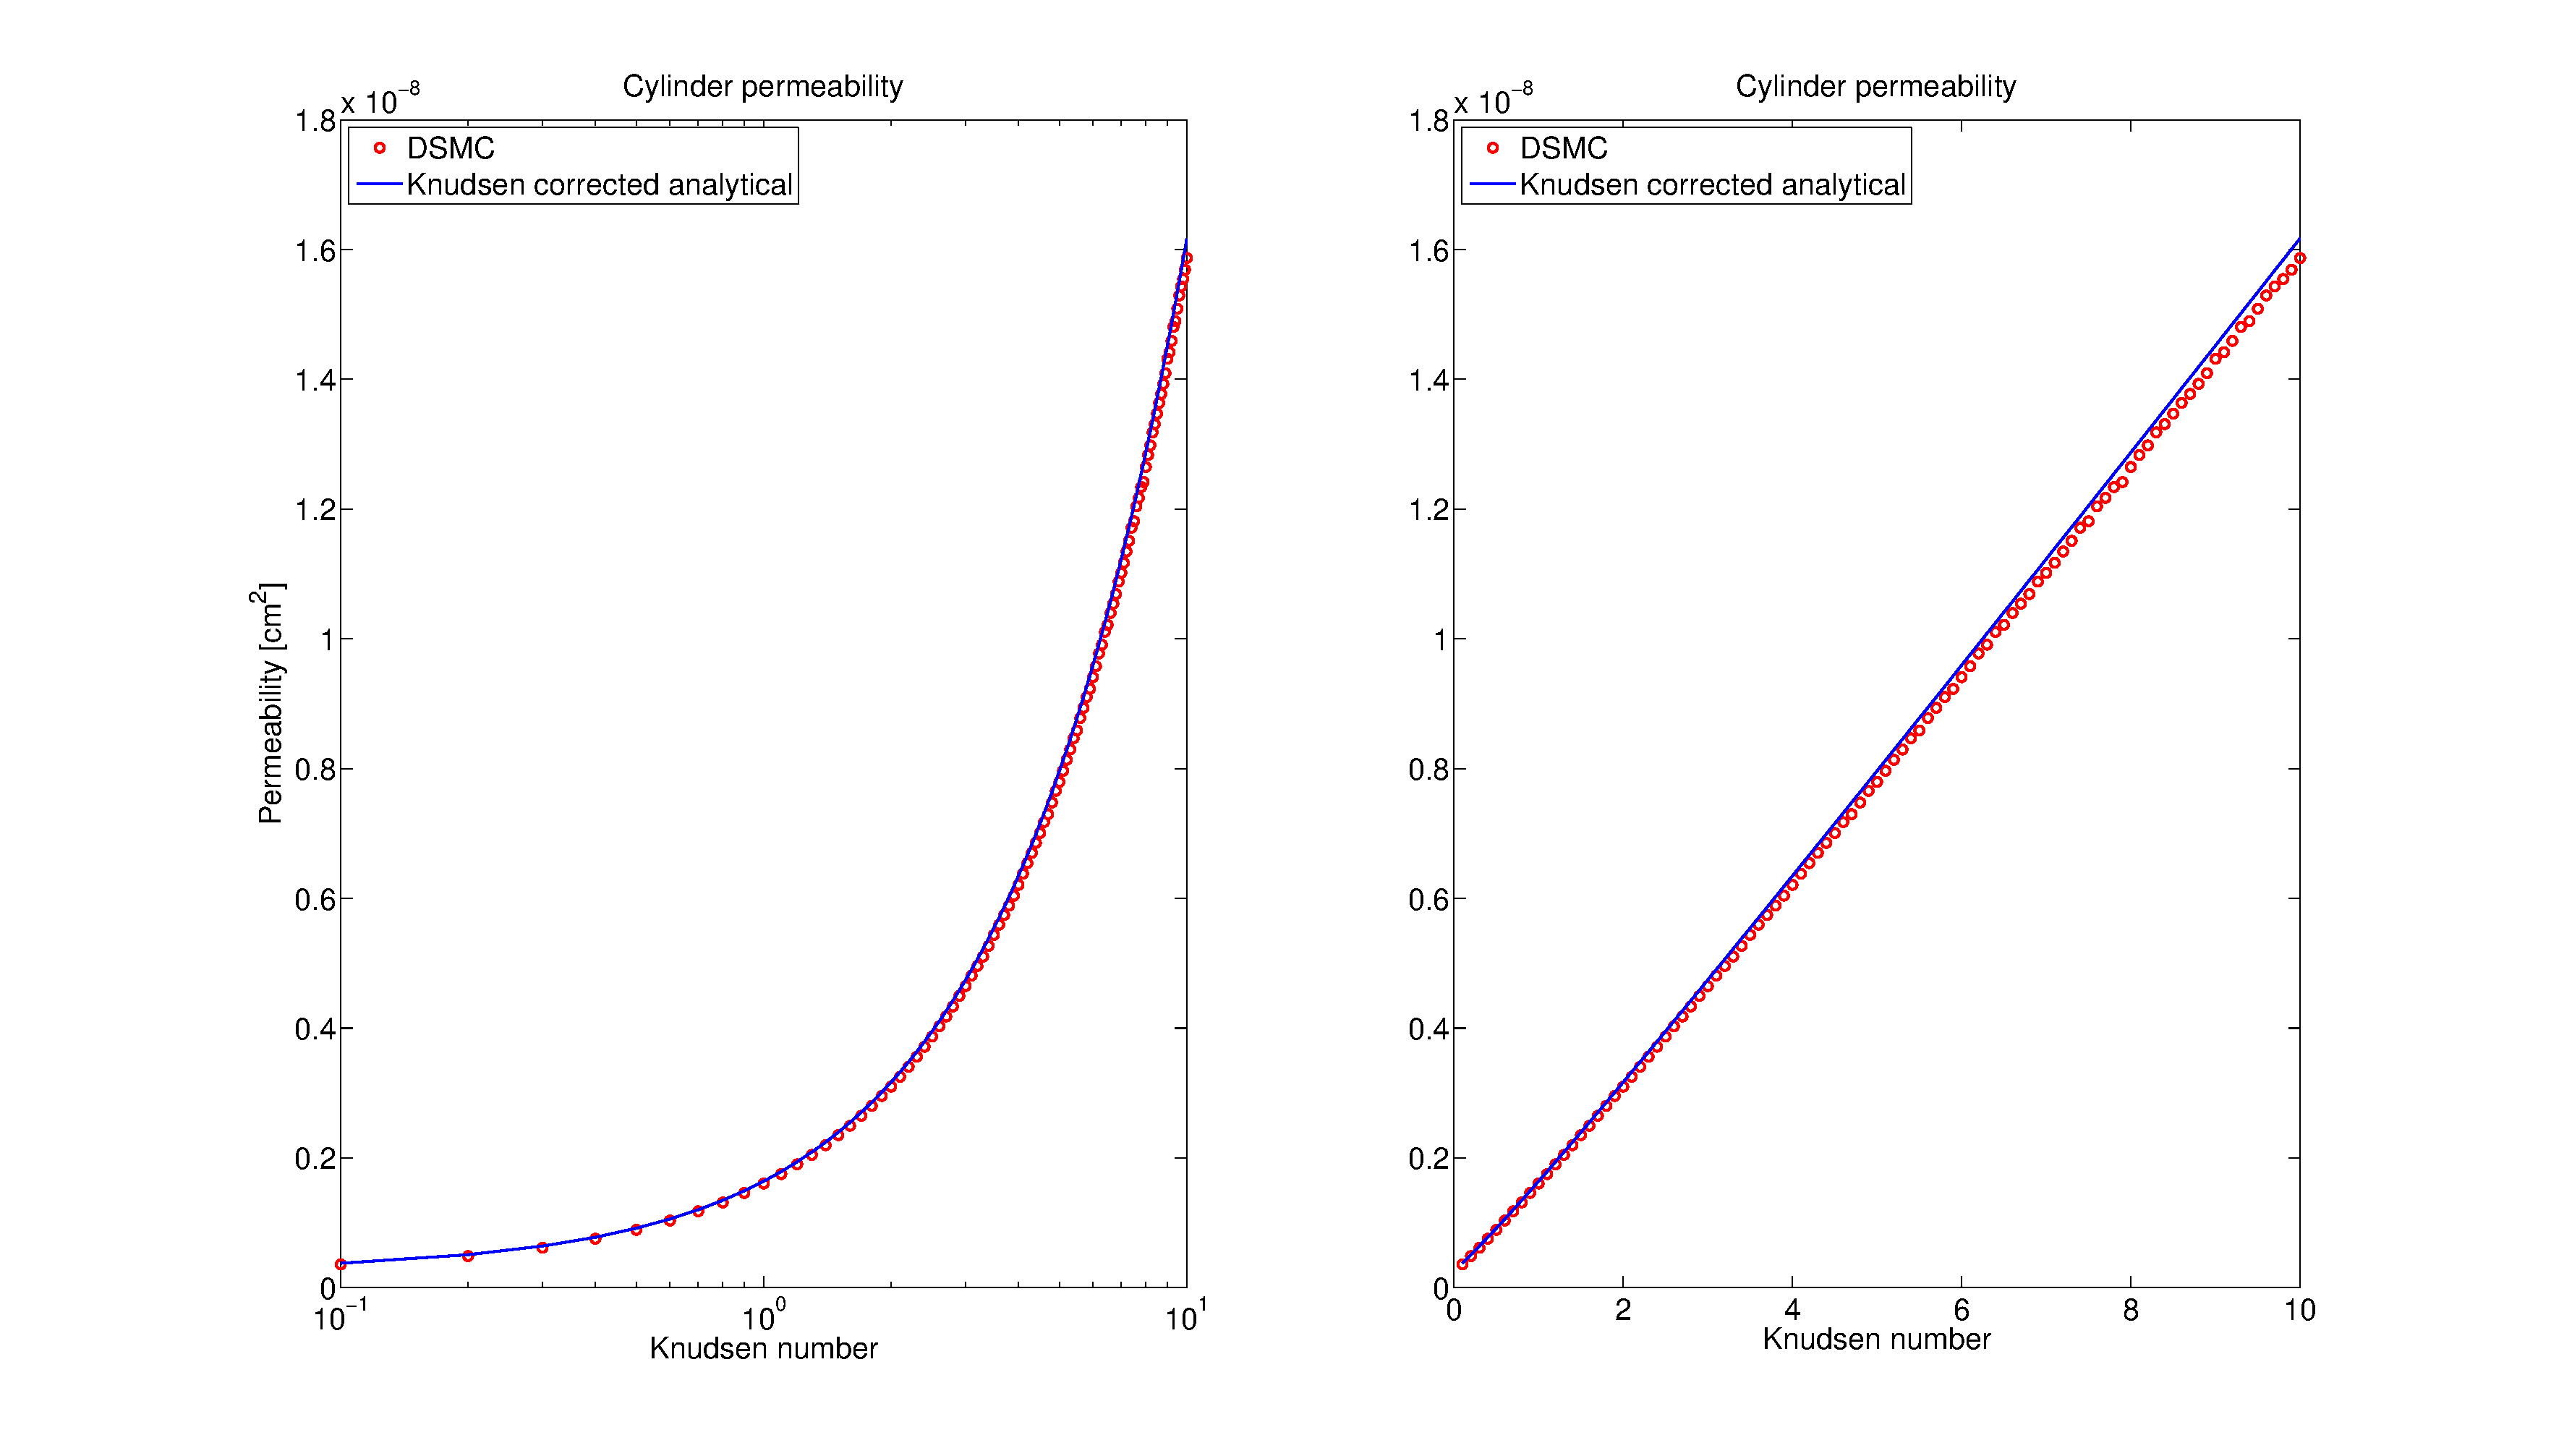
\includegraphics[width=\textwidth, trim=0cm 0cm 0cm 0cm, clip]{DSMC/figures/cylinder_knudsen_permeability.eps}
\end{center}
\caption{Permeability as a function of Knudsen number for a cylinder with radius \unit{0.45}{\micro\meter} and length \unit{1}{\micro\meter} with an applied pressure difference $\Delta P = 1.1P_0$ ($P_0$ being the ideal gas pressure). We control the Knudsen number by varying the density. The blue line is the Knudsen corrected analytical solution from \cite{karniadakis2005microflows}. The DSMC results confirm that the Knudsen correction factor works very well for a system with a well defined Knudsen number.}
\label{fig:one_cylinder_varying_knudsen}
\end{figure}

\subsection{Flow in a cylinder, varying radius}
If we instead keep the Knudsen number constant ($\text{Kn}=1.0$), we can vary the radius to verify equation \eqref{eq:permeability_cylinder}. We have studied radii in the range \unit{0.1}{\micro\meter} to \unit{0.45}{\micro\meter} with the same pressure difference as in the previous simulation ($\Delta P = 1.1P_0)$. In figure \ref{fig:one_cylinder_varying_radii_result} we have plotted the measured permeability as a function of cylinder radius. The straight line confirms the quadratic dependency in equation \eqref{eq:permeability_cylinder}.
\begin{figure}[h]
\begin{center}
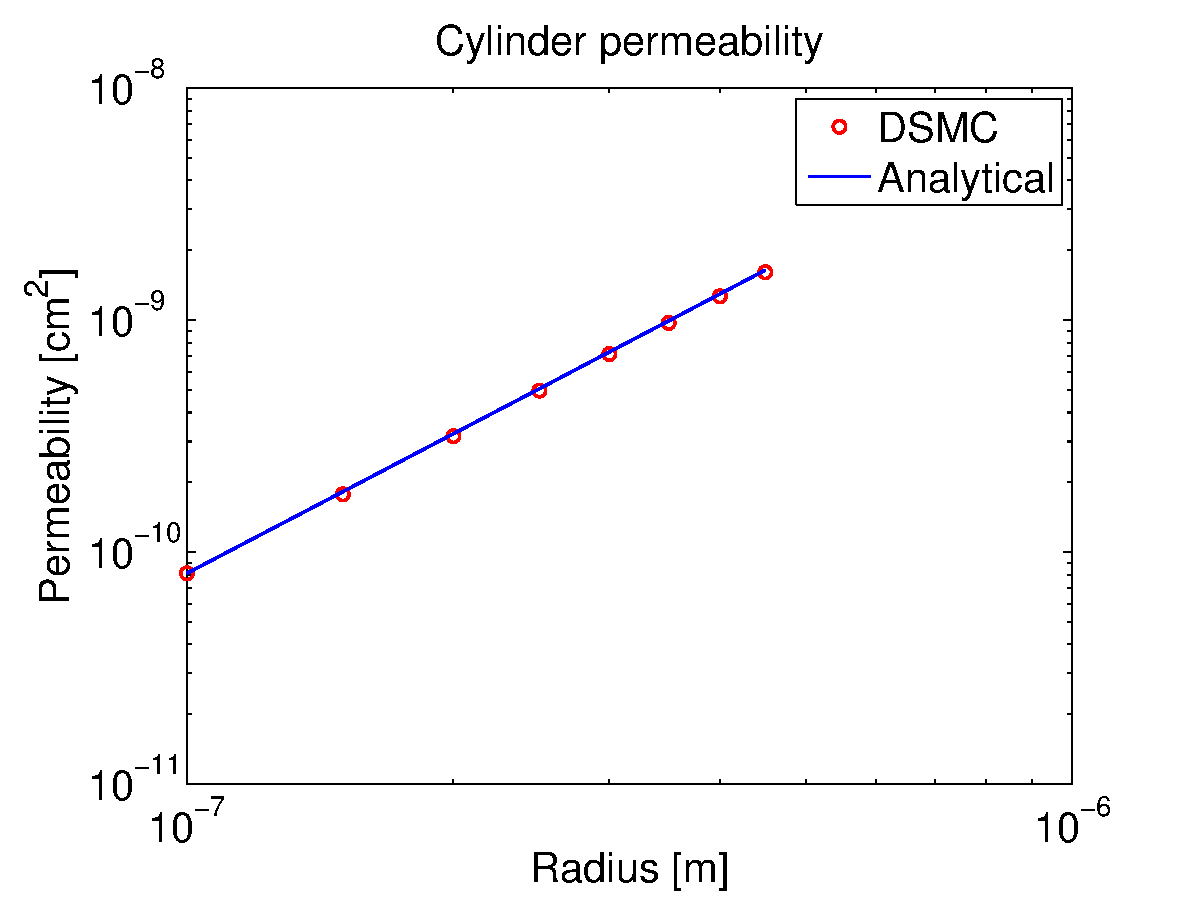
\includegraphics[width=\textwidth, trim=0cm 0cm 0cm 0cm, clip]{DSMC/figures/cylinder_radius_permeability.eps}
\end{center}
\caption{Logarithmic plot of the permeability for different cylinders with radii in the range $0.1 \mu m$ to $0.45 \mu m$ with an applied pressure difference $\Delta P = 0.1P_0$. The blue line is the Knudsen corrected analytical solution from \cite{karniadakis2005microflows}.}
\label{fig:one_cylinder_varying_radii_result}
\end{figure}

\section{Results for complicated geometries}
\label{sec:dsmc_packed_spheres_results}
We have now seen that the Knudsen correction factor works well for systems with a well defined Knudsen number. It does however need \textit{one} Knudsen number to be able to predict the permeability, but for more complex geometries, there is rather a distribution of Knudsen numbers than a single number. It could work as a lower and an upper limit of the permeabilities for two different input Knudsen numbers, but they could possibly differ by an order of magnitude. Another approach could be to find the average distance $\langle L\rangle$ to the surface and use that distance to estimate the Knudsen number as
\begin{align}
    \text{Kn}^* = \frac{\lambda}{\langle L \rangle}.
\end{align}
In this section we will study a system consisting of randomly packed spheres  that does not have a well defined Knudsen number. The spheres may overlap, so their positions are completely independent of each other. The distribution and expectation value of distances to sphere surfaces is derived in appendix \ref{app:knudsen_number_packed_spheres} also providing a suggestion to the estimated Knudsen number $\text{Kn}(r,\phi)^*$ for packed spheres of radius $r$ and porosity $\phi$. First we discuss the Carman-Kozeny equation which is an analytical expression for the permeability for packed spheres. Then we discuss how the simulation is run and discuss the result.
\subsection{The Carman-Kozeny equation}
In 1927, Kozeny proposed an equation predicting the (absolute) permeability of packed spheres of radius $r$ forming a system with porosity $\phi$ given as
\begin{align}
	k_\infty = {r^2 \over 9K} {\phi^3 \over (1 - \phi)^2},
\end{align}
where $K$ is the Kozeny constant which is experimentally measured to be around five for equally size spheres\cite{carman1937fluid}. This result has been verified to predict permeabilities in many macro scale experiments since its discovery. However, at the nanometer scale, we expect deviations due to high Knudsen numbers. Using the Knudsen correction factor with the estimated Knudsen number $f_c(\text{Kn}(r,\phi)^*)$ (equations \eqref{eq:knudsen_correction} and \eqref{eq:packed_sphere_estimated_knudsen}), we expect the permeability to be
\begin{align}
    k_a(r) = f_c\left[\text{Kn}(r,\phi)^*\right]{r^2 \over 9K} {\phi^3 \over (1 - \phi)^2}.
\end{align}
\subsection{The simulation and results}
We ran the simulation for spheres with radii from \unit{0.01}{\micro\meter} to \unit{0.08}{\micro\meter} while keeping approximately constant porosity, $\phi\approx 0.3$. This was done by adding spheres until the desired porosity was obtained. For each radius, ten geometries were created with different seeds yielding better statistics. The permeability for each sphere radius is then averaged over the ten different geometries. In figure \ref{fig:packed_spheres_permeability}, we have plotted the permeabilities measured in the simulations with the average value of the ten runs per sphere radius. We have also plotted the Knudsen corrected Carman-Kozeny permeability which gives a pretty good estimate for the permeability. 
\begin{figure}[h]
\begin{center}
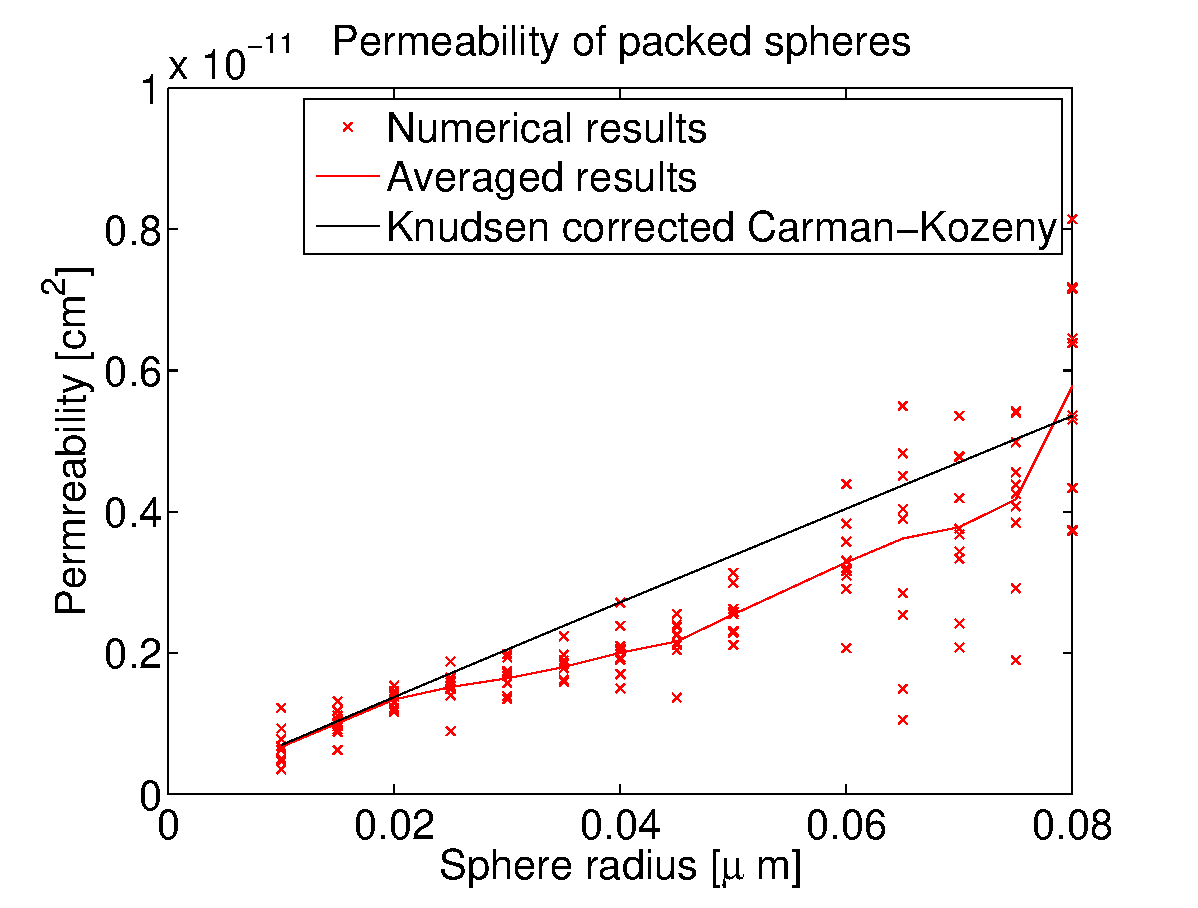
\includegraphics[width=\textwidth, trim=0cm 0cm 0cm 0cm, clip]{DSMC/figures/permeability_packed_spheres.eps}
\end{center}
\caption{Permeability for different sphere radii in a system consisting of packed spheres. The red dots show the numerical results whereas the red line shows the average value for each sphere radius. The black line is the Knudsen corrected Carman-Kozeny expression for the permeability with the estimated Knudsen number (equation \eqref{eq:packed_sphere_estimated_knudsen}). We see that due to the large statistical spread in the sphere configurations, the spread in permeability is also quite large. While the Knudsen corrected Carman-Kozeny expression does give a good estimate of the permeability, it is clear when the spread in Knudsen numbers is large, it is not sufficient with one single average value.}
\label{fig:packed_spheres_permeability}
\end{figure}